\section{سوال اول}
در بخش‌های مختلف سوال به بررسی عملکرد قانون هدایت خط دید\LTRfootnote{Line Of Sight}
بررسی شده است.
\subsection{بخش الف}
در این بخش شبیه‌سازی موشک و هدف به مدت ۱۰ ثانیه انجام شده است. نتایج شبیه‌سازی در ادامه آورده شده است.

\begin{figure}[H]
	\centering
	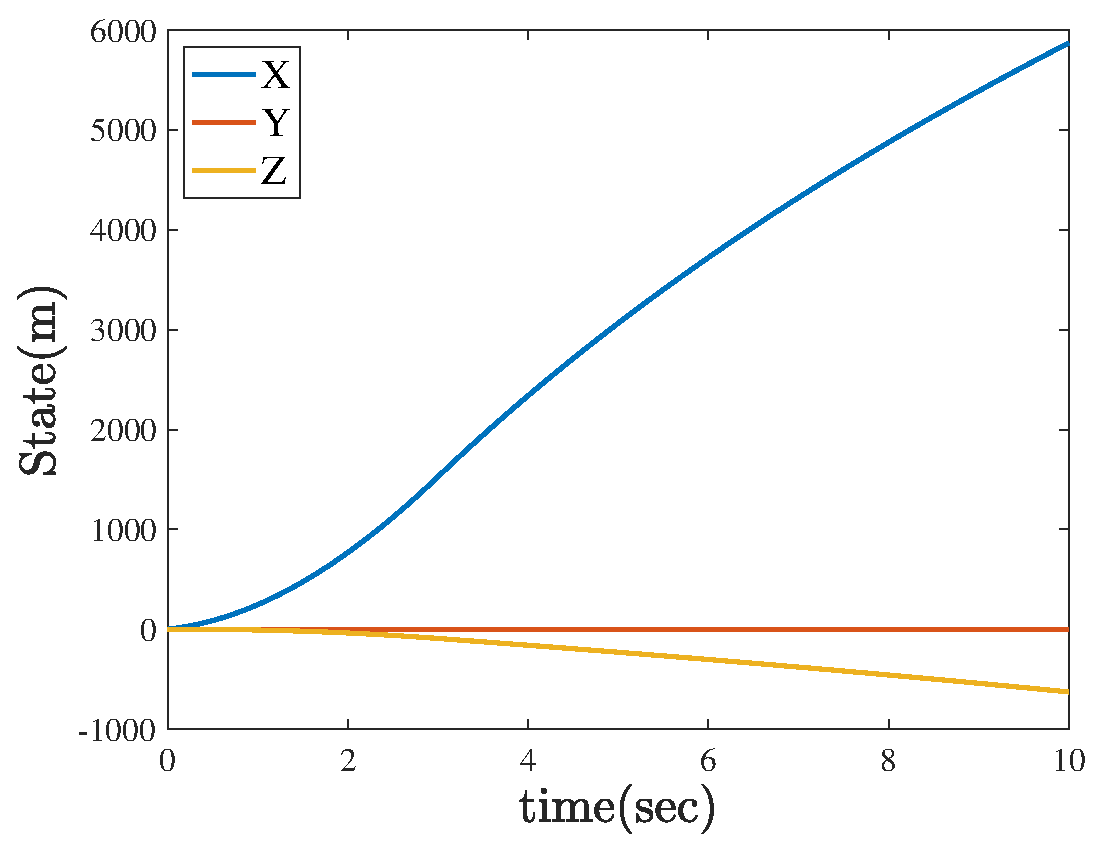
\includegraphics[width=.75\linewidth]{../Figure/a/missle_state}
	\caption{موقعیت موشک}
\end{figure}

\begin{figure}[H]
	\centering
	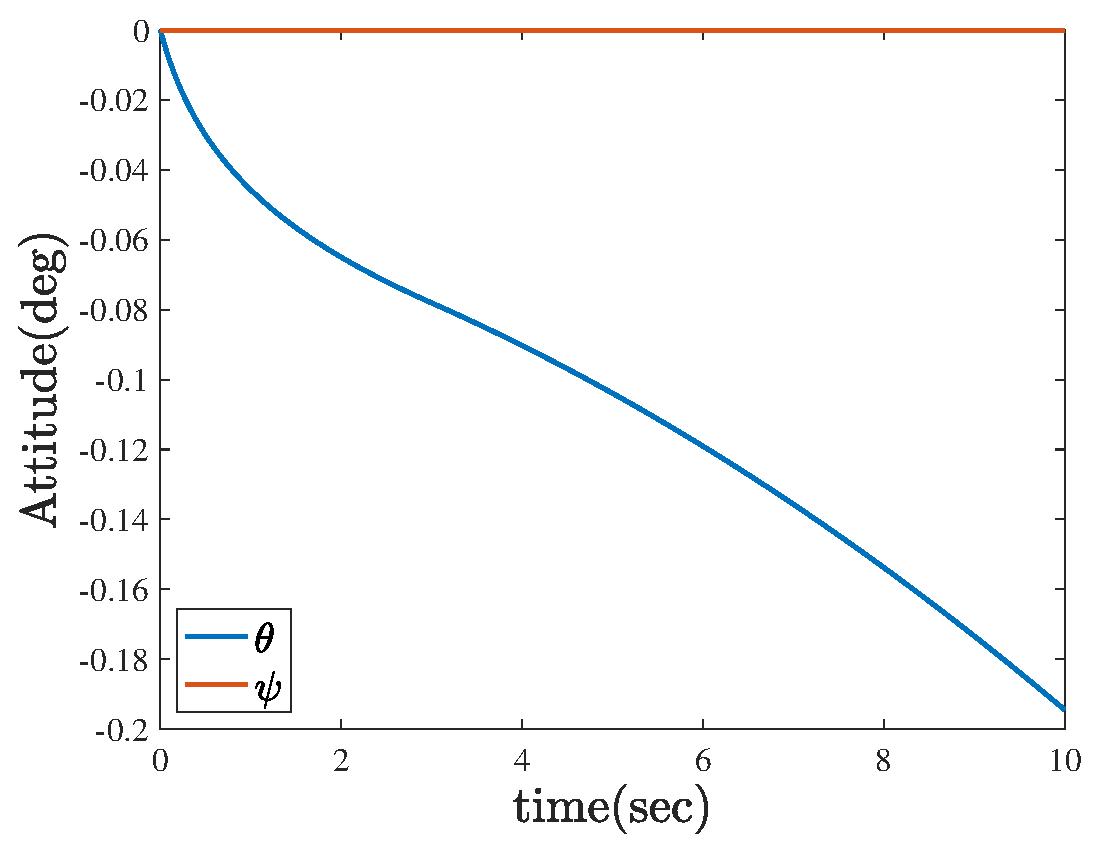
\includegraphics[width=.75\linewidth]{../Figure/a/missle_attitude}
	\caption{وضعیت موشک}
\end{figure}

\begin{figure}[H]
	\centering
	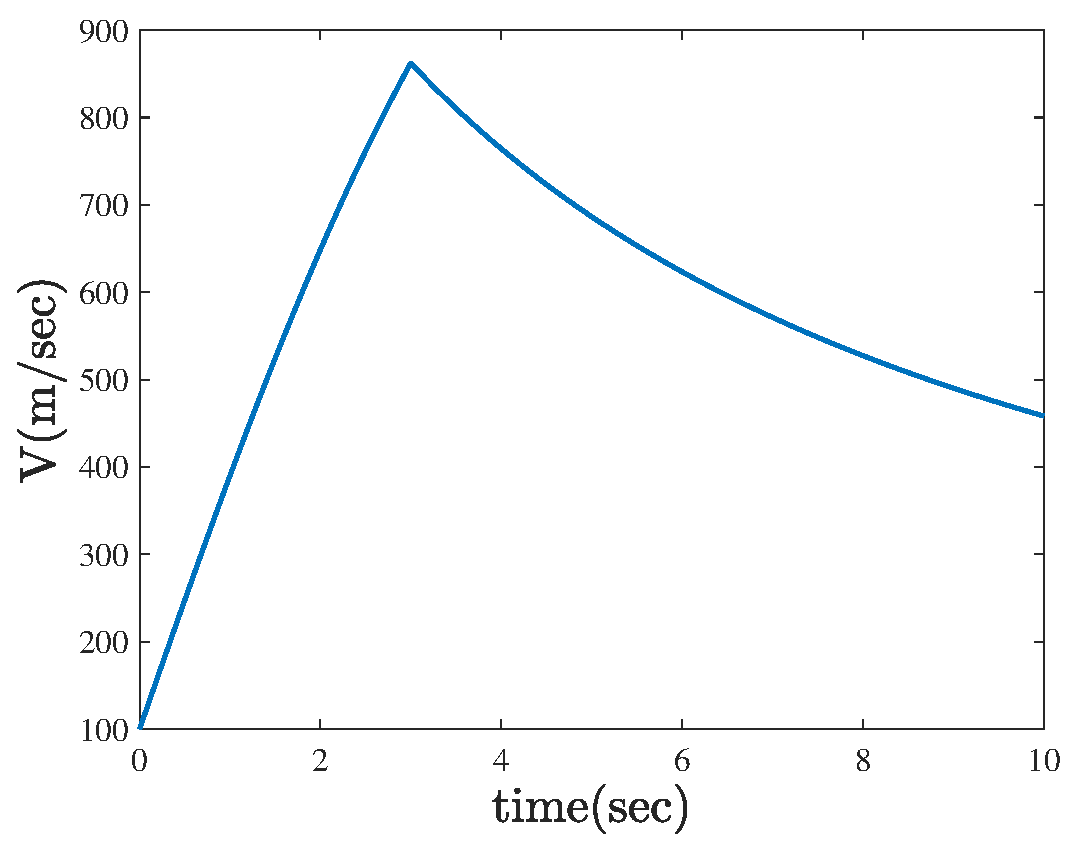
\includegraphics[width=.75\linewidth]{../Figure/a/missle_V}
	\caption{سرعت موشک}
\end{figure}

\begin{figure}[H]
	\centering
	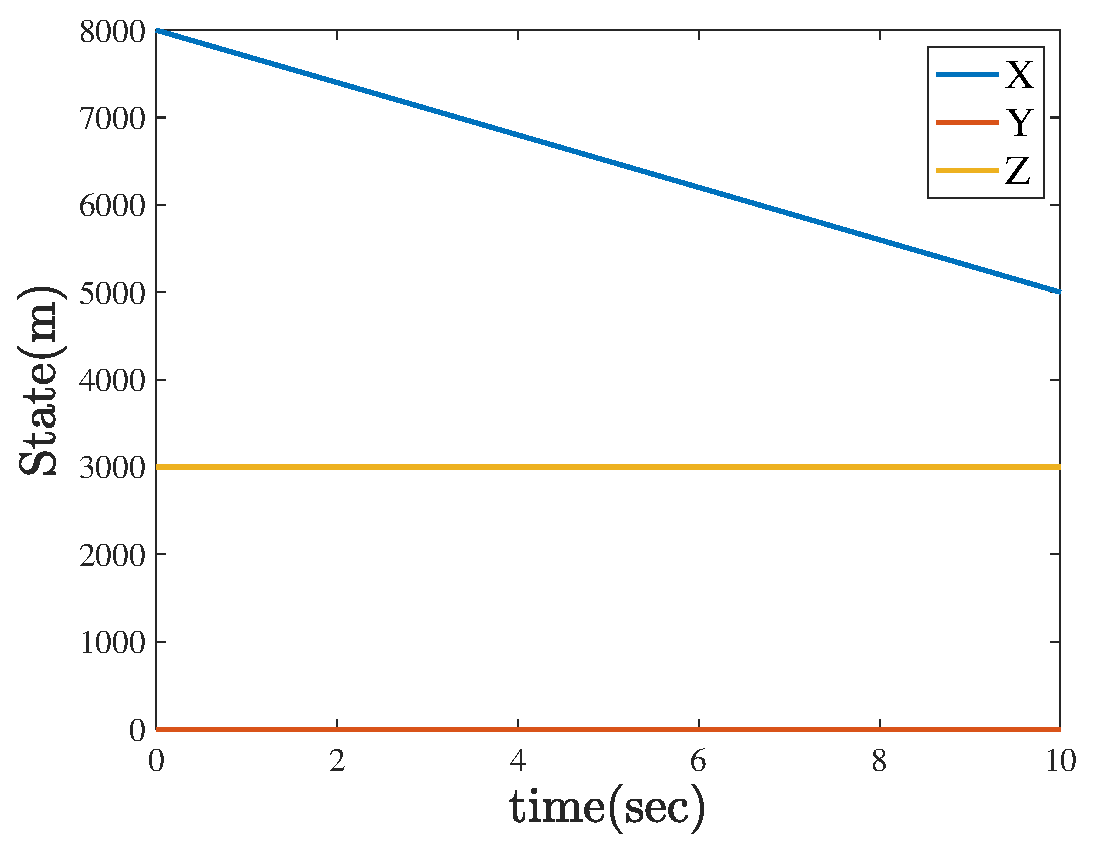
\includegraphics[width=.75\linewidth]{../Figure/a/target_state}
	\caption{موقعیت هدف}
\end{figure}

\begin{figure}[H]
	\centering
	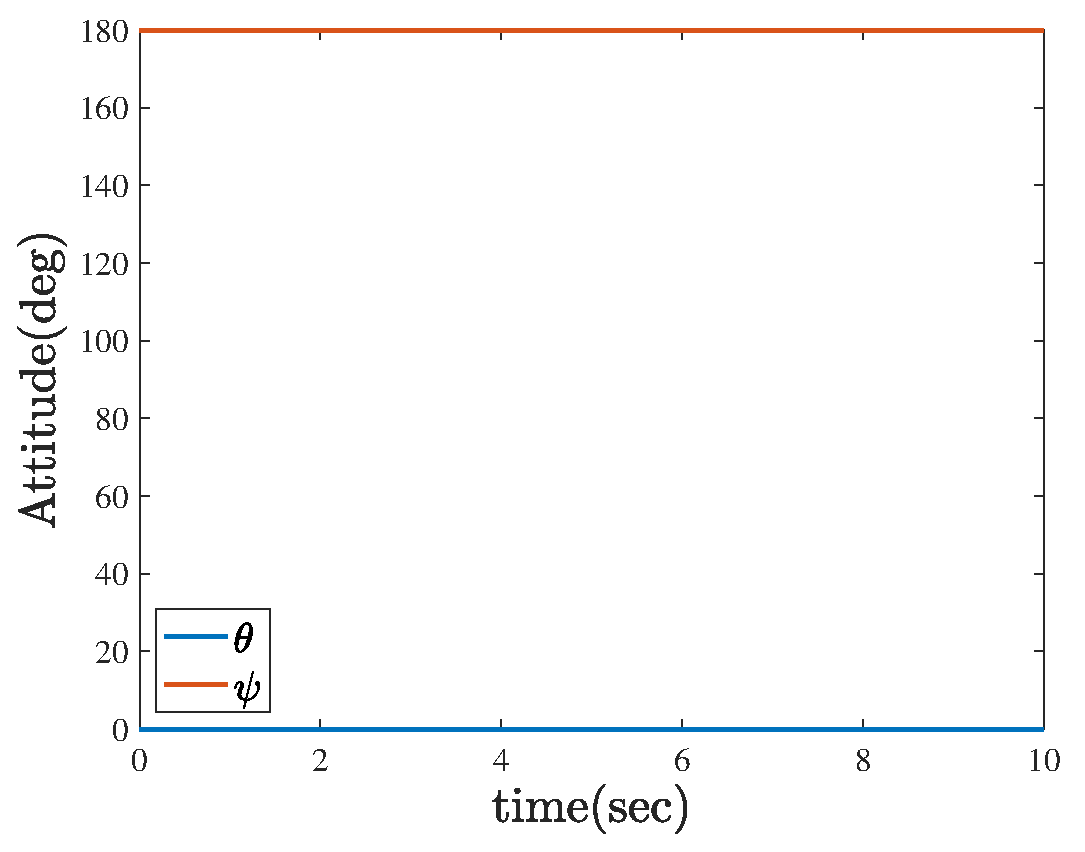
\includegraphics[width=.75\linewidth]{../Figure/a/target_attitude}
	\caption{وضعیت هدف}
\end{figure}

\begin{figure}[H]
	\centering
	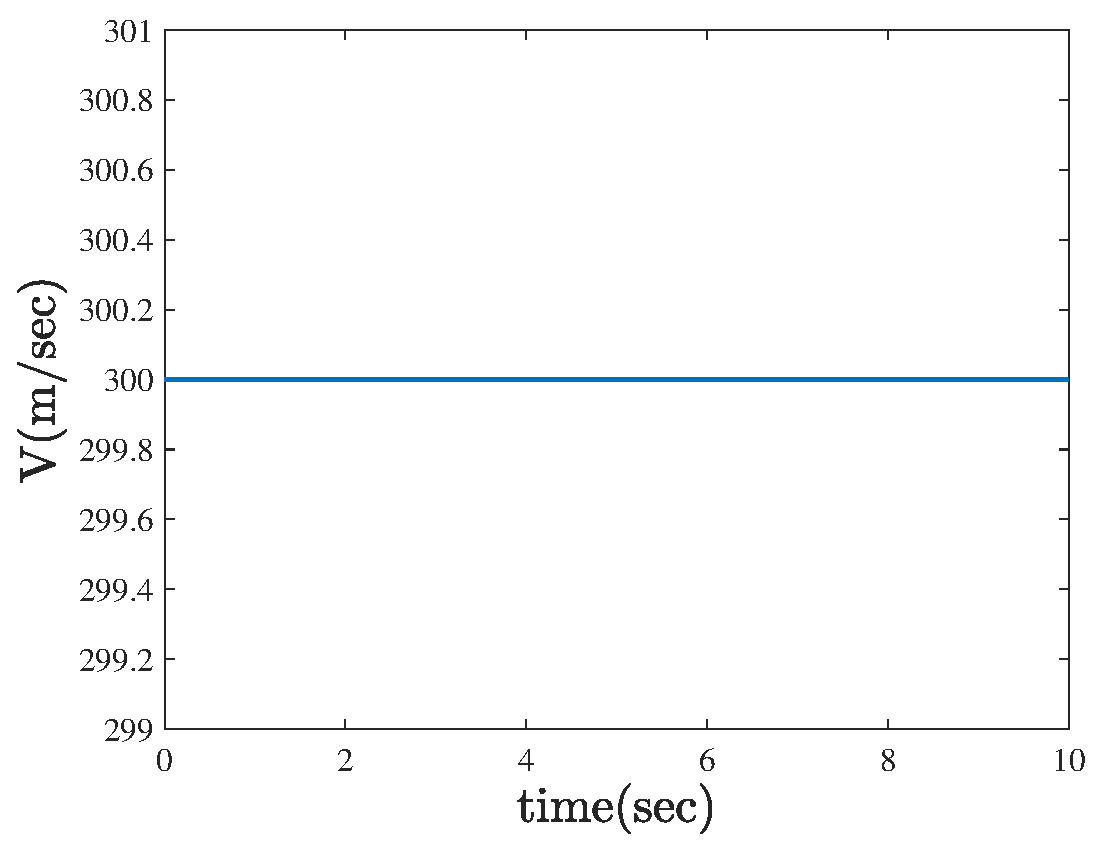
\includegraphics[width=.75\linewidth]{../Figure/a/target_V}
	\caption{سرعت هدف}
\end{figure}


